\documentclass[tikz,border=10pt]{standalone}
\usetikzlibrary{calc}
\begin{document}
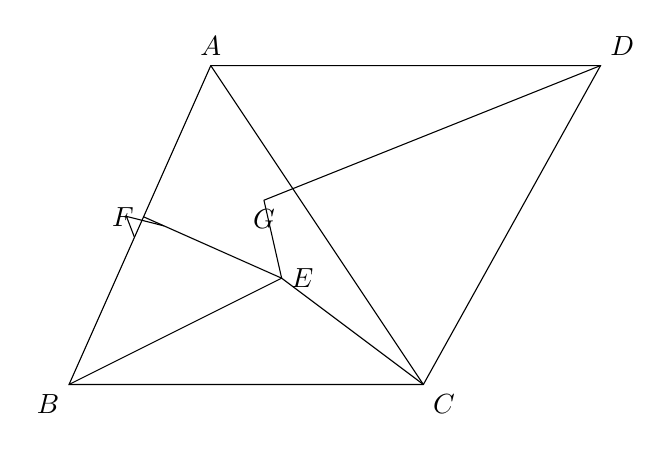
\begin{tikzpicture}[scale=0.9]
  \coordinate (B) at (0,0);
  \coordinate (C) at (5,0);
  \coordinate (D) at (7.5,4.5);
  \coordinate (A) at (2,4.5);
  \coordinate (E) at (3,1.5);
  \coordinate (F) at ($(A)!(E)!(B)$);
  \coordinate (G) at (2.75,2.6);
  \draw (A) -- (B) -- (C) -- (D) -- cycle;
  \draw (A) -- (C);
  \draw (B) -- (E) -- (C);
  \draw (E) -- (F);
  \draw (E) -- (G);
  \draw (G) -- (D);
  % right-angle mark at F
  \draw ($(F)!9pt!(B)$) -- ($($(F)!9pt!(B)$)!9pt!90:($(F)!9pt!(E)$)$) -- ($(F)!9pt!(E)$);
  \node[above] at (A) {$A$};
  \node[below left] at (B) {$B$};
  \node[below right] at (C) {$C$};
  \node[above right] at (D) {$D$};
  \node[right] at (E) {$E$};
  \node[left] at (F) {$F$};
  \node[below] at (G) {$G$};
\end{tikzpicture}
\end{document}
